% Metódy inžinierskej práce
% !TEX TS-program = pdflatexmk

\documentclass[10pt,english,a4paper]{article}

\usepackage[english]{babel}
%\usepackage[T1]{fontenc}
\usepackage[IL2]{fontenc} % lepšia sadzba písmena Ľ než v T1
\usepackage[utf8]{inputenc}
\usepackage{graphicx}
\usepackage{url} % príkaz \url na formátovanie URL
\usepackage{hyperref} % odkazy v texte budú aktívne (pri niektorých triedach dokumentov spôsobuje posun textu)
\usepackage {lipsum}
\usepackage{cite}
\usepackage{subfig}
\usepackage{wrapfig}
\usepackage{amsmath}

%\usepackage{times}

\pagestyle{headings}

\title{Comparison of Blockchain usage in different sectors\thanks{Semestral project in subject Metods of Engineering work, ac. year 2023/2024}} % meno a priezvisko vyučujúceho na cvičeniach

\author{Zdenko Kanoš\\[2pt]
	{\small Slovak University of Technology in Bratislava}\\
	{\small Faculty of Informatics and Information Technologies}\\
	{\small \texttt{xkanos@stuba.sk}}
	}

\date{\small 28.09.2023} % upravte



\begin{document}

\maketitle

\begin{abstract}
To clarify my framework topic, I'll start with the name of my article: “Comparison of
blockchain usage in different sectors”. In my perspective, blockchain represents the future
of secure data storage, particularly for classified documents. The primary aim of my article is
to emphasize blockchain’s current and future utility. I was inspired by enlightening articles
highlighting blockchain's practical application in various real-world scenarios. These articles
paved my way to focus on sectors like police records, decentralized voting, or how
government data can be stored on the blockchain. In my article, I will also talk about why
storing data on the blockchain is better and more secure and what is different about the
application of blockchain in different sectors.
\end{abstract}

\section{Sekcia 1}
 \lipsum[1-3]
  \begin{figure}
  \centering
   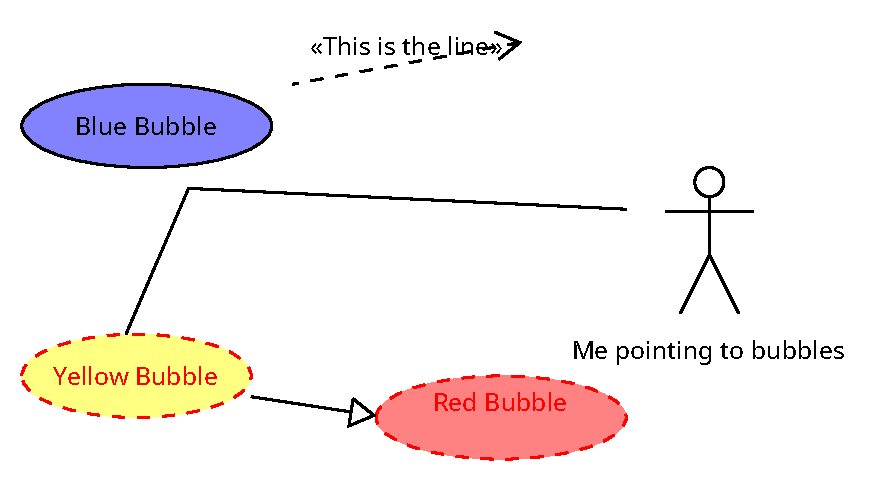
\includegraphics[scale=0.8]{Diagram_1.pdf}
  \centering
  \caption{Diagram}
 \end{figure}
 \lipsum[1-2]
 
 \begin{figure}%
    \centering
    \subfloat[\centering label 1]{{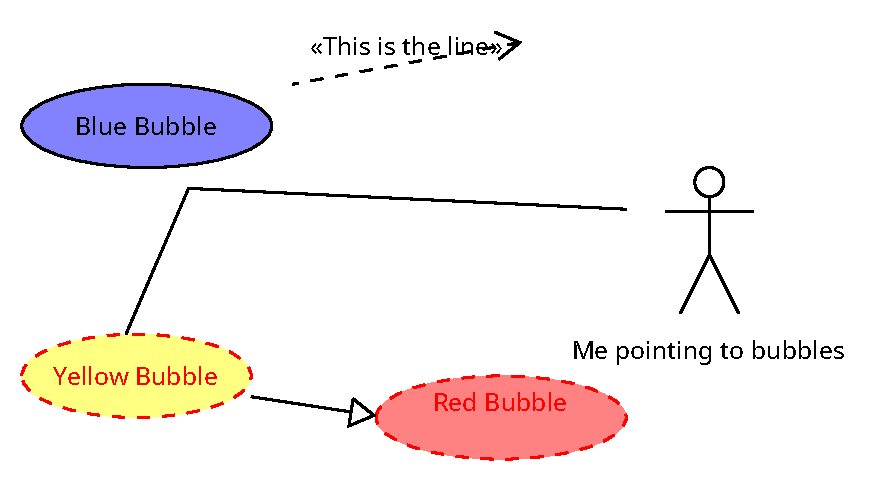
\includegraphics[width=5cm]{Diagram_1.pdf} }}%
    \qquad
    \subfloat[\centering label 2]{{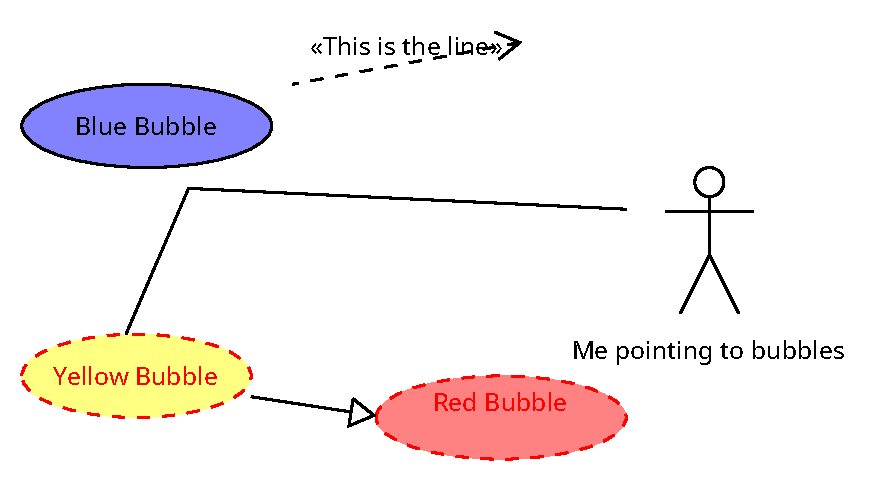
\includegraphics[width=5cm]{Diagram_1.pdf} }}%
    \caption{2 Figures side by side}%
    \label{fig:example}%
\end{figure}
 
 \lipsum[1-3]

 \section{Sekcia 2}
 \lipsum[1-2]
 \begin{wrapfigure}{r}{0.5\textwidth}
  \centering
  
\includegraphics[width=0.48\textwidth]{STU-FIIT-ancv.png} % replace with your actual file name
  \caption{Test Diagram}
\end{wrapfigure} 
 \lipsum[1-4]
 
$\begin{bmatrix}
  a & b & c & d & e &f\\
  g & h & i & j & k &l \\
  m & n & o & p & r &s\\
   a & b & c & d & e &f\\
  g & h & i & j & k &l \\
  m & n & o & p & r &s\\

  
\end{bmatrix}$



 
 
% týmto sa generuje zoznam literatúry z obsahu súboru literatura.bib podľa toho, na čo sa v článku odkazujete
\bibliography{literatura}
\bibliographystyle{alpha} % prípadne alpha, abbrv alebo hociktorý iný
\end{document}
